\section{Processing of Two Subject-Verb Dependencies in NLMs and Humans}
The core mechanism to carry agreement information across long-range dependencies in NLMs involves a very small number of units--one (Italian) or two (English). This mechanism was shown to robustly process sentences having a single long-range dependency. We next ask: given that the long-range agreement mechanism is sparse, and can thus only encode a single number feature at a time, how will the NLM process \emph{two} long-range dependencies that are active at once?

Two simultaneously active long-range dependencies occur in various constructions, such as center-embedded nested dependencies, a prototypical example of recursion. In nested dependencies, once the long-range agreement mechanism is engaged in tracking the main dependency, there may be no more suitable units available to process the \textit{embedded} agreement. For example, in the sentence ``The \textbf{boy} that the \textit{farmer} near the \underline{fathers} \textit{watches} \textbf{knows} the daughters'', there are two grammatical numbers that need to be carried across a long-range dependency: (1) that of the main subject `boy', and (2) that of the embedded subject `farmer'. Once the NLM  encounters the main subject, its grammatical number can be stored through the long-range agreement mechanism up to the main verb `knows'. However, during this period, since the mechanism is already taken up, once the embedded subject `farmer' is presented to the network, there is no robust way to encode and carry its number up to the embedded verb `watches'. The NLM is thus predicted to fail to process the embedded dependency in nested structures.

We emphasize two conditions for this predicted failure:
\begin{APAitemize}
	\item The two dependencies are \textit{simultaneously} active at some point: if this is not the case, i.e., the dependencies are successive (e.g., ``The \textbf{boy} near the \underline{cars} \textbf{says} that the \textit{farmer} near the \underline{fathers} \textit{watches} the daughters''), the long-range mechanism can first complete processing the first dependency, and then reset before encoding the next one. 

    \item Both dependencies are \textit{long-range}: in the case
          of a short-range dependency nested within a long-range one
          (e.g., ``The \textbf{boy} that the \textit{farmer}
          \textit{watches} \textbf{knows} the daughters''), the
          embedded short-range dependency can still be processed by
          the short-range units we described above, although possibly in a less robust way compared to the main dependency. 
\end{APAitemize}

We next present the experimental design we used to confirm these predictions about the NLM, as well as to test whether they also extend to human subjects, which would suggest that the agreement processing system of the latter bears similarities to the one we uncovered in NLMs.

\subsection{Experimental Design}
To test the hypothesis that the sparsity of the long-range mechanism can lead to a significant processing difficulty at the embedded dependency, we created a two-by-two design that manipulates the above two conditions: (1) whether the two dependencies are \textit{successive} or \textit{nested}, and (2) whether the embedded dependency is \textit{short} or \textit{long} range. 
Figure \ref{fig:design} describes the resulting four NA-tasks: Short-Successive, Long-Successive, Short-Nested and Long-Nested (`Short' and `Long' therefore refer to the length of the embedded dependency only). 

The successive tasks serve as control. They minimally differ from the nested ones up to the embedded verb, by only a single word (`dice' (`says') in Figure \ref{fig:design}). Note also that tasks that have a long embedded dependency have a third noun, which functions as a possible attractor, inside the embedded dependency. We will refer to this most-deeply embedded noun as the `inner attractor', although note that the subjects of the main and nested clauses can also act as attractors on each others' verbs.

For each NA-task, we generated various \textit{conditions} by varying the number of the main and embedded subject noun, and that of the attractor. Short-Successive and Short-Nested have each four conditions corresponding to the possible assignments of number to the main and embedded subjects - SS, SP, PS and PP. Similarly, Long-Successive and Long-Nested have eight conditions, based on the possible numbers of the main, embedded subject and attractor - SSS, SSP, SPS, etc. In what follows, by \textit{congruent subjects} we refer to conditions in which the main and embedded subjects share grammatical number (SS, PP, SSS, SSP, PPS and PPP), and by \textit{incongruent subjects} to the rest (SP, PS, SPS, etc.). By \textit{congruent attractor}, we refer to conditions in which the embedded subject and the third noun share grammatical number (SSS, SPP, PSS and PPP), and by \textit{incongruent attractor} to conditions in which they differ (SSP, SPS, PSP, PPS) (Table \ref{tab:na-tasks-overview}).

Several studies reported markedness effects in agreement, whereby humans make more errors when the grammatical number of the attractor is plural. This effect was reported in several languages and in both comprehension and production (\textit{English}: \citet{Bock:Miller:1991, eberhard1997marked, wagers2009agreement}; \textit{Italian}: \citet{vigliocco1995constructing}; \textit{Spanish}: \citet{bock2012number, lago2015agreement}; \textit{French}: \citet{franck2002subject}; \textit{Russian}: \citet{lorimor2008agreement}). Since we use error rates as an index of processing difficulties across various conditions, we strove to increase their overall signal. Therefore, we first present all analyses on contrasts with a plural attractor.
Results for the full set of conditions, with both singular and plural attractors, are reported subsequently.

Table \ref{tbl:predictions} summarizes our predictions for each task and structure, while ignoring for now, for ease of presentation, differences among specific conditions. 
For Short- and Long-Successive, no significant processing difficulties are predicted, since the long-range mechanism can encode the main and nested grammatical numbers sequentially. 
For Short- and Long-Nested, the long-range mechanism is predicted to successfully process the main dependency and therefore no significant difficulties are predicted on the main verb (beyond the relative difficulty to process center-embeddings reported for both humans \citep{traxler2002processing} and NLMs \citep{marvin2018targeted}). In contrast, the embedded dependency in Short-Nested cannot rely on the long-range agreement mechanism, as it is recruited by the main dependency. Consequently, the processing of the embedded dependency can only rely on short-range mechanisms, which might not be as robust as the long-range ones. We are thus agnostic about success in this case. Finally, in Long-Nested, the performance on the embedded verb is predicted to be significantly low, given that the long-range mechanism can process only a single agreement, as described above.

\begin{center}
\begin{table}
\centering
\begin{tabular}{|P{3.5cm}||P{3.5cm}|P{3.5cm}|}
    \hline
    \B Sentence Type & \B Main Verb & \B Embedded Verb \\
    \hline
    Successive-Short & V  & V \\
    \hline
    Successive-Long & V & V \\
    \hline
    Nested-Short & V & - \\
    \hline
    Nested-Long & V & X \\
    \hline
\end{tabular}
\caption{A summary of the predictions of model performance on successive and nested dependencies based on the sparsity of the long-range mechanism. 'V' and 'X' represent high and low predicted performance on the agreement task, respectively. Due to possible compensation mechanisms carried by the short-range number units, we make no precise predictions regarding performance on the embedded verb of Nested-Short.}
\label{tbl:predictions}
\end{table}
\end{center}

\begin{figure}[ht]
    \centering
    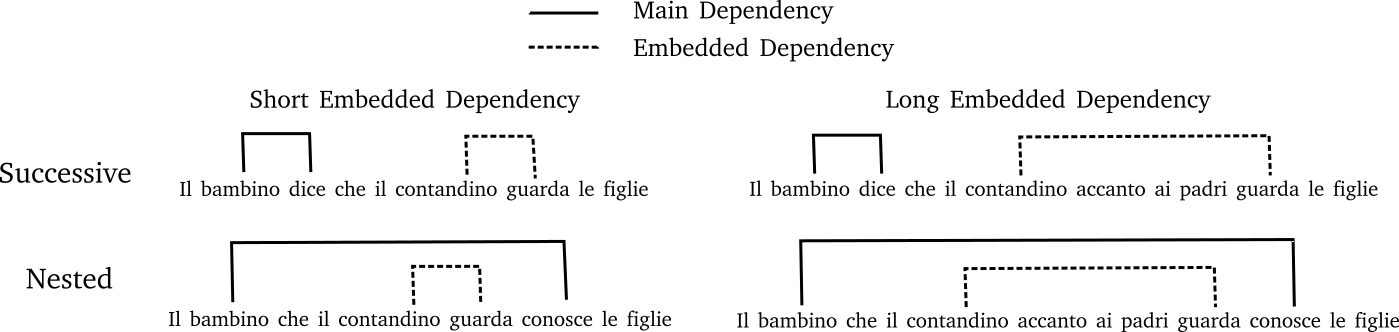
\includegraphics[width=\textwidth]{figures/design.png}
    \caption{\textbf{A full-factorial design for two subject-verb dependencies}. Human subjects and Neural Language Models were presented with sentences from four different syntactic structures, which all have two subject-verb dependencies: a main dependency (continuous lines) and an embedded dependency (dashed). The first factor of the design determines whether the two dependencies are \textit{successive} (top structures) or \textit{nested} (bottom), depending on whether the structure has a sentential complement or an object-extracted relative clause, respectively. The second factor determines whether the embedded dependency is \textit{short} (left side) or \textit{long} (right). We refer to the four resulting structures as: Short-Successive, Long-Successive, Short-Nested and Short-Long.}
    \label{fig:design}
\end{figure}

\begin{figure}[ht]
    \centering
    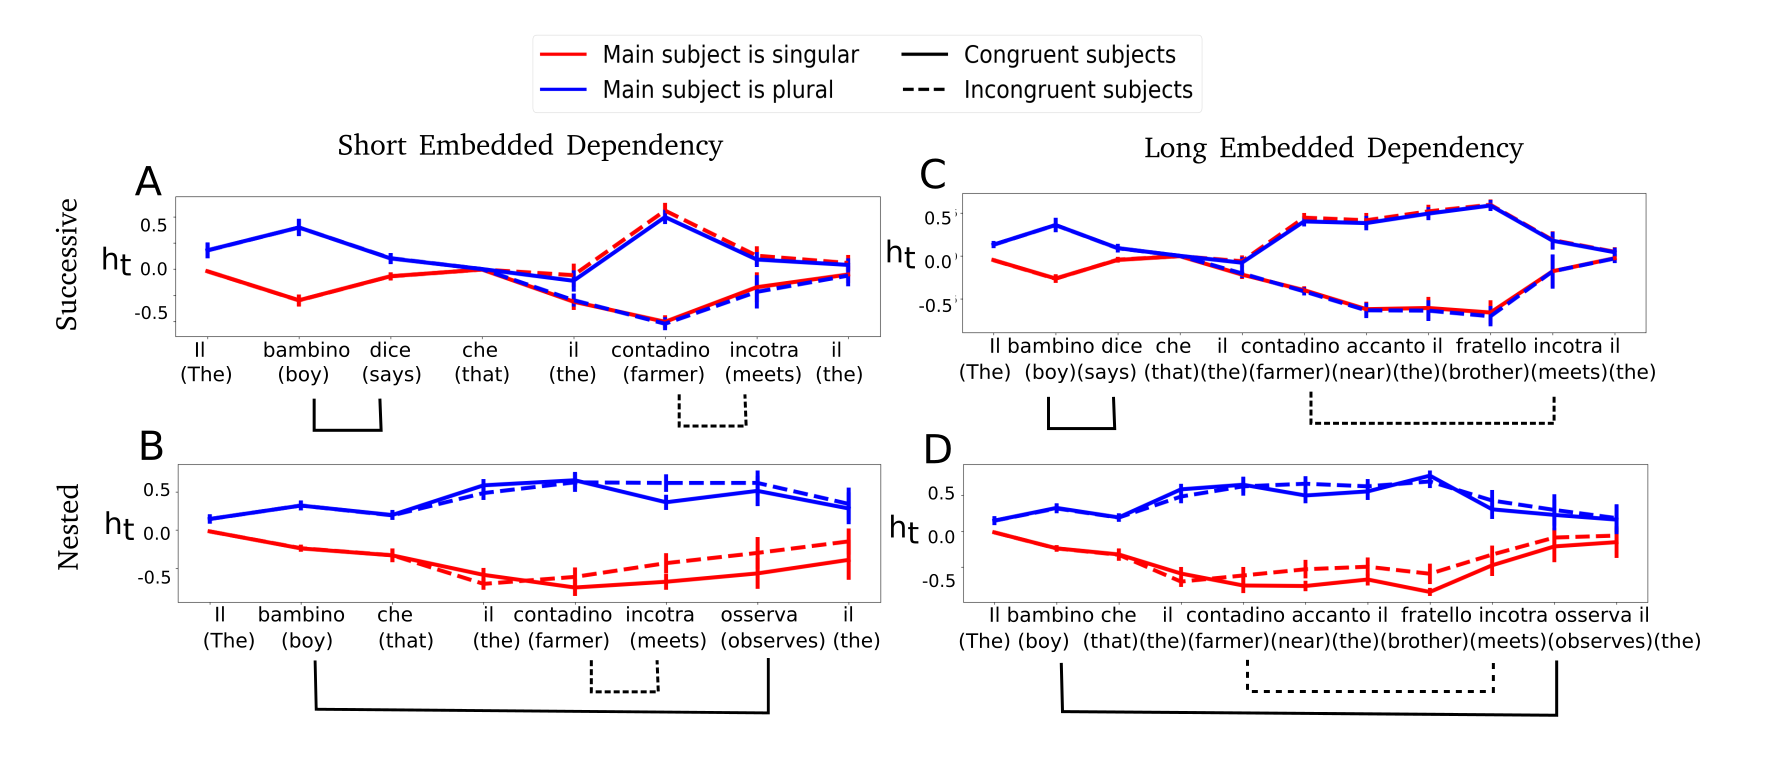
\includegraphics[width=\textwidth, clip, trim={0mm 0mm 0mm 0mm}]{figures/model_activations_2by2.png}
    \caption{\textbf{Dynamics of the activity of the number unit during the processing of two subject-verb dependencies.} Number-unit activity is presented for the four structures in the design: Short-Successive (panel A), Long-Successive (B), Short-Nested (C) and Long-Nested (D). For each structure, results are presented for four conditions, corresponding to whether the main subject of the sentence is singular (red curves) or plural (blue), and to whether the main and embedded subjects have the same grammatical number (congruent; continuous lines) or not (incongruent; dashed lines). (A) \textit{Short-Successive}: the number unit processes the two successive dependencies sequentially. After the encoding of the first subject ('bambino'), activity return to baseline (around zero) before encoding the embedded subject ('contadino'). (B) \textit{Long-Successive}: a similar sequential encoding is observed also when the embedded dependency is long-range. (C) \textit{Short-Nested}: the number unit carries the grammatical number of the main subject ('bambino') up to the main verb ('evita'), also in conditions in which the embedded subject and verb carry opposite gammatical number (dashed lines). (D) \textit{Long-Nested}: encoding of the grammatical number of the main subject is robust also when the embedded dependency is long-range.}
    \label{fig:2by2_dynamics}
\end{figure}



\subsection{Methods and Materials for the Simulations with the NLM}
We used four different Number-Agreement tasks (NA-tasks, bottom, Table~\ref{tab:na-tasks-overview}). All tasks contain two subject-verb dependencies, which differ in terms of whether they are \emph{successive} or \emph{nested} and whether the embedded dependency is \emph{short-} or \emph{long-range}. Two subject-verb dependencies are \emph{successive} when the second subject occurs only after the first has been resolved. 
Such dependencies occur, for instance, in declarative sentences with a sentential complement, such as ``Il \textbf{ragazzo} \textbf{dice} che la \textit{donna conosce} il cane'' (``The \textbf{boy says} that the \emph{woman knows} the dog'').
In this example, the subject and verb are directly adjacent in both dependencies.
We thus call these dependencies \emph{short-range}, and the above sentence is an example of a sentence that could occur in the \emph{Short-Successive} NA-task. 
To create sentences that have a successive but \emph{long-range} subject-verb relationship, we increase the distance between the second noun and its corresponding verb by inserting a prepositional phrase in between: ``Il \textbf{ragazzo} \textbf{dice} che la \textit{donna} accanto al \underline{figlio} \textit{conosce} il cane' '(``The \textbf{boy says} that the \emph{woman} next to the \underline{son} \emph{knows} the dog''). For nested dependencies, we consider sentences with object-relative clauses, such as ``Il \textbf{ragazzo} che la \emph{figlia} \emph{ama} \textbf{conosce} il contadino'' (``The \textbf{boy} who the \emph{daughter} \emph{loves} \textbf{knows} the farmer'').
As the nested dependency in this sentence is short range, we call the corresponding number-agreement task \emph{Short-Nested} (note however that the main-clause dependency is long range). For \emph{Long-Nested}, we again use prepositional phrases to increase the distance between the subject and verb of the nested dependency: ``Il \textbf{ragazzo} che la \emph{figlia} vicino alla \underline{donna} \emph{ama} \textbf{conosce} il contadino'' (``The \textbf{boy} who the \emph{daughter} near the \underline{woman} \emph{loves} \textbf{knows} the farmer'').

For each NA-task, we generated 4096 sentences that were randomly sampled from a fixed lexicon (Table \ref{tbl:lexicon}). The performance of the model on each condition was then evaluated in the same way as described in section \ref{sss:model_eval}.

\subsection{Results for the Italian NLM}\label{results_NLMs}
\subsubsection{The Number Unit Shows Sequential Processing of Two Successive Dependencies and Robust Encoding of the Main Dependency in Nested Constructions}
We first simulated NLM dynamics for all NA-tasks and conditions, by presenting all sentences from each condition to the NLM. Figure \ref{fig:2by2_dynamics} presents hidden-state dynamics of the long-range number unit during the processing of all conditions from the four NA-tasks. We note that, consistent with results on a single dependency, the grammatical number of the main subject is encoded with the same polarity as found in the NounPP task - positive for plural (blue) and negative for singular (red). Second, in successive NA-tasks, the activation of the number unit returns to baseline after encountering the main verb (`dice'), and then rises back once the embedded subject is encountered. This shows that the number unit can sequentially encode two grammatical numbers in two successive dependencies, also when the two numbers are opposite. In particular, note that in Long-Successive, the grammatical number of the embedded subject is robustly carried across the attractor (`fratello') in the incongruent conditions (dashed lines). Finally, in both Short- and Long-Nested, the grammatical number of the main subject is robustly carried across the main dependency up to the main verb (`osserva'), and in particular, across the embedded subject and verb that carry an opposite number in some conditions (dashed lines).

\subsubsection{NLM Performance on Successive Dependencies}
Since no significant processing difficulty is predicted in the successive tasks, we conducted the experiments on the embedded agreement only, which is expected to be the more difficult one. 
This allowed us to reduce experimental duration in the parallel study with human participants. Also, to facilitate the interpretation of the results, we grouped conditions by whether the main and embedded subjects were congruent or not.

Figure \ref{fig:error_rates_plural_attractor}A presents the resulting NLM error rates (Figure \ref{fig:error_rates_all_conditions} further provides the full error-rate distribution across all conditions). Several effects are observed in the results: 

\begin{APAitemize}
    \item \textbf{Near perfect performance on all conditions}: Overall, for both Short- and Long-Successive, the performance of the NLM was found to be almost error free, with slightly more errors in the Long-Successive case ($z=26.3, p<0.001$)
    \item \textbf{Subject-congruence effect}: We next tested for a \textit{subject-congruence effect}, i.e., whether incongruent subjects elicited more errors compared to congruent ones. We found a significant subject-congruence effect in both Short- and Long-Successive (Short-Nested: $z=5.4, p<0.001$; Long-Nested: $z=6.4, p<0.001$). Note that the variance of the network is very low, which renders this effect significant, although the error rate is near zero in both congruent and incongruent cases.
\end{APAitemize}
 
 \begin{figure}[ht]
    \centering
    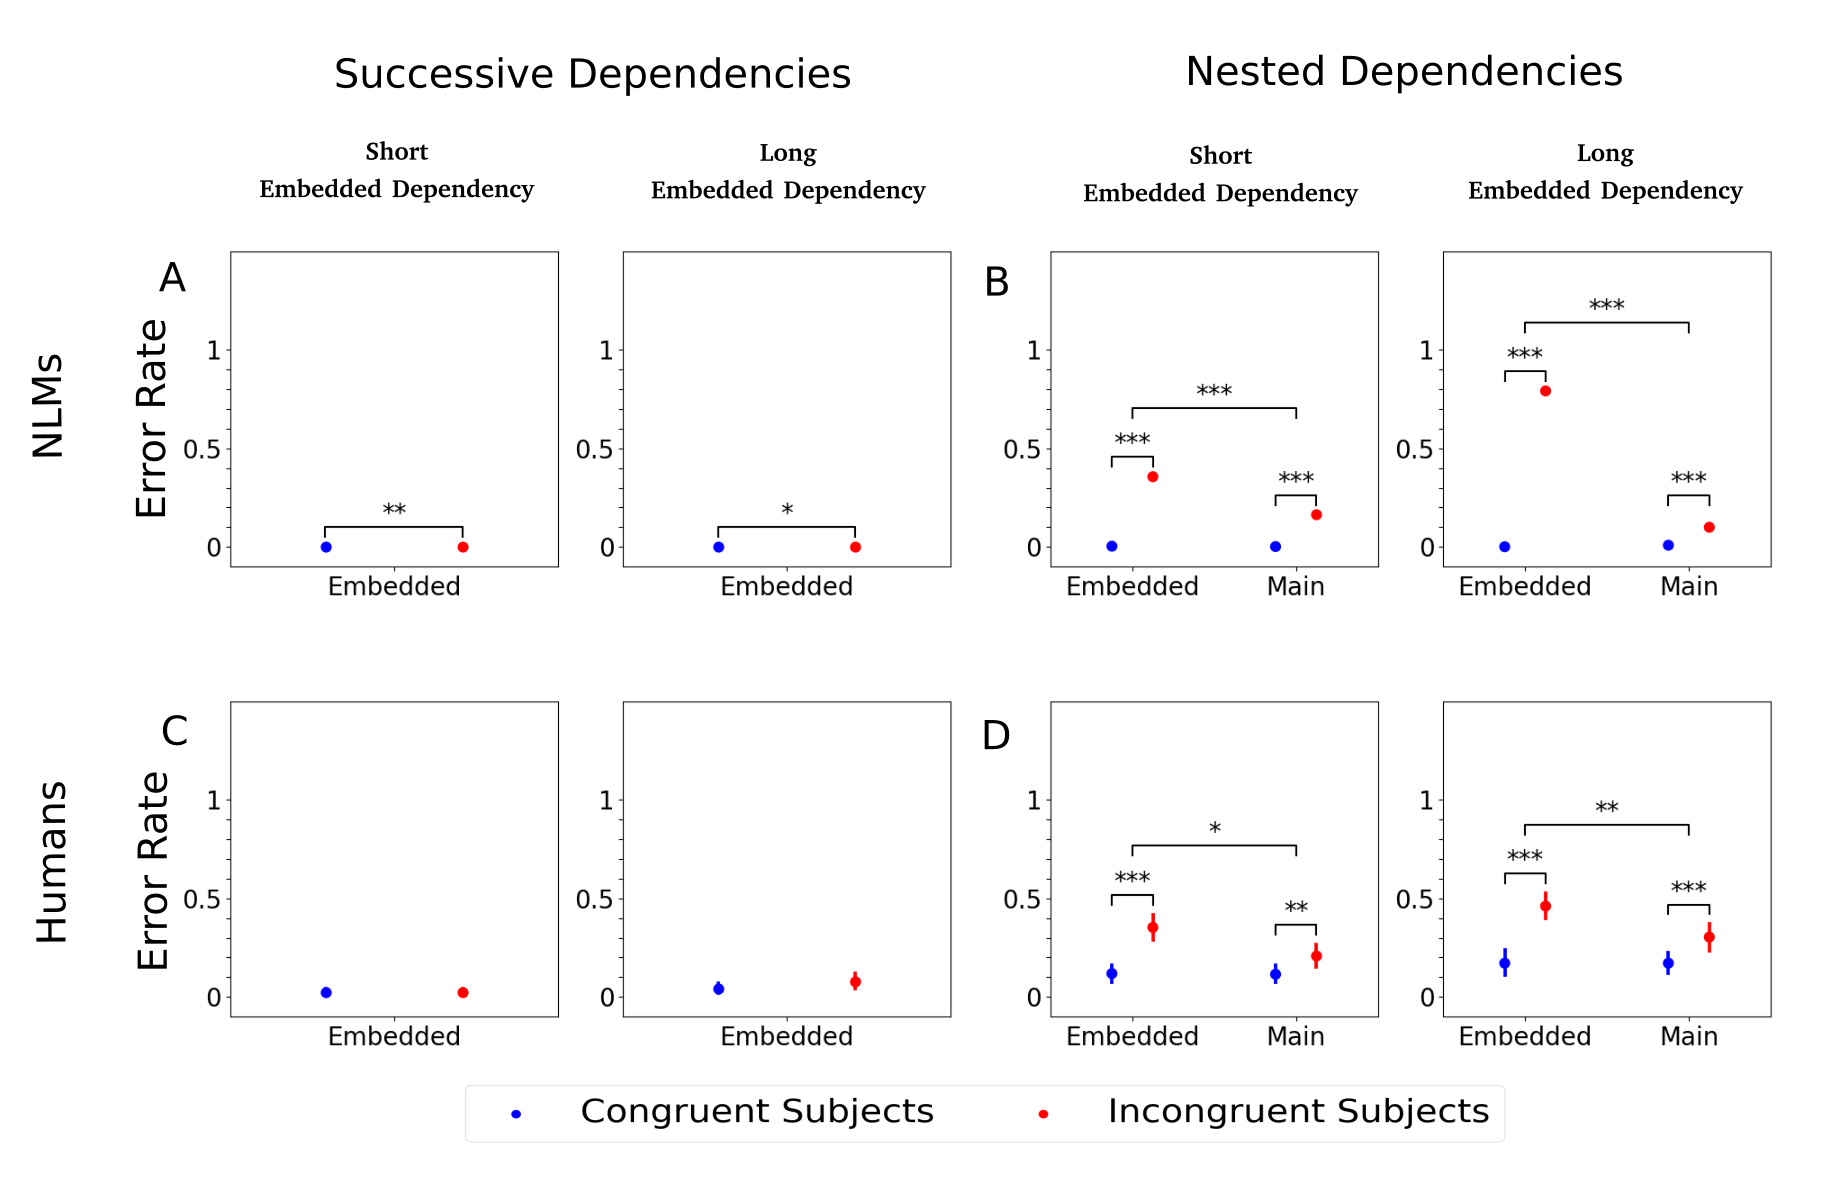
\includegraphics[width=16cm]{figures/error_rates_plural_attractor.png}
    \caption{\textbf{Comparison of error rates} predicted by the Neural Language Model (top, panels A \& B) and observed in human participants (bottom, panels C \& D). Blue and red colors correspond to whether the main and embedded subjects agree on number (congruent subjects) or not (incongruent), respectively. Error bars represent the 95\% confidence level.}
    \label{fig:error_rates_plural_attractor}
\end{figure}


\subsubsection{NLM Performance on Nested Dependencies}
Figure \ref{fig:error_rates_plural_attractor}B presents the corresponding error rates in the case of nested dependencies (Figure \ref{fig:error_rates_all_conditions} further provides the full error-rate distribution across all conditions). Several effects are observed in the results:

\begin{APAitemize}
    \item \textbf{Incongruent conditions elicit more errors}: a significant subject-congruence effect was found on both the embedded and main verbs, in both Short- and Long-Nested (Short-Nested main: $z=93.1, p<0.001$; Short-Nested embedded: $z=50.9, p<0.001$; Long-Nested main: $z=67.0, p<0.001$; Long-Nested embedded: $z=120.5, p<0.001$). In all cases, incongruent subjects elicited more errors compared to congruent subjects.
    \item \textbf{Processing of embedded verbs is more error-prone}: for both Short- and Long-Nested, a significant interaction was found between subject-congruence and verb-position (embedded/main), with a larger increase of error rate due to incongruent subjects on the embedded compared to the main verb (Short-Nested: $z=32.3, p<0.001$; Long-Nested: $z=84.2, p<0.001$).
    \item \textbf{A longer embedded dependency is more error prone}: for errors made on the embedded verb, we found a significant interaction between subject-congruence and the length of the embedded dependency (Short/Long-Nested), with a larger increase of error rate due to incongruent subjects in Long-Nested ($z=7.4, p<0.001$).
\end{APAitemize}
 
\vspace{10pt}

\subsubsection{Discussion of NLM results}
Focusing on cases with incongruent subjects, the error patterns of the NLM are overall consistent with the predictions summarized in Table \ref{tbl:predictions}. First, successive dependencies are relatively easy for the model, and can be processed sequentially. This is consistent with the sequential encoding observed in the dynamics of the number unit (Figure \ref{fig:2by2_dynamics}), which shows a robust encoding of grammatical number of embedded subjects, also in the presence of an attractor. Second, the main dependency in both Short- and Long-Nested was successfully processed (i.e., significantly better than chance level), although with more overall errors compared to successive dependencies. Third, the NLM made an exceptionally large number of errors on the embedded verb in Long-Nested, as predicted by the sparsity of the long-range mechanism. This is prominent in the case of incongruent-subject, since only then the grammatical number of the main subject encoded in the long-range mechanism can interfere. Finally, the NLM made a relatively large number of errors on the embedded verb in Short-Nested but was significantly better than chance level ($error \quad rate = 0.5$; $p-value < 0.001$). The reduced number of errors in Short- compared to Long-Nested is consistent with the findings about a less sophisticated short-range mechanism that can process the embedded dependency, compensating for the momentary recruitment of the long-range mechanism for the main one. 

\subsection{Methods and Materials for the Behavioral Experiment with Humans}
\subsubsection{Participants}
61 psychology students from the University of Milano-Bicocca (males = XX; Age = XX ± XX; Education = XX ± XX \YL{@Alessandra}) took part in the experiment in exchange for course credits. 
Participants were Italian native speakers and were naive with respect to the experiment purpose. 
The study was approved by the ethical committee of the Department of Psychology, and ethical treatment was in accordance with the principles stated in the Declaration of Helsinki.

\subsubsection{Stimuli}
Stimuli comprised i) acceptable sentences; ii) violation trials, which contained a number violation on the verb of one of the subject-verb agreements; iii) filler sentences, comprising several syntactic and semantic violations. 

Acceptable sentences were created using a pool of 10 nouns, 19 verbs, 4 prepositions (Table \ref{tbl:lexicon}), for all four main constructions (bottom, Table~\ref{tab:na-tasks-overview}). Starting from this pool of sentences, number-violation and filler trials were created by replacing either the main or embedded verb by the opposite form of the verb with respect to number. For example, ``il \textbf{fratello} che lo \emph{studente *accolgono} \textbf{ama} i contadini'' (``the \textbf{brother} that the \emph{student *welcome} \textbf{loves} the farmers'').

Filler trials contained either a semantic or syntactic violation that does not concern number. 
Syntactic violations were generated by either, \begin{APAitemize}\setlength\itemsep{0mm}
\item [i)] replacing a verb with a wrong person without changing number, for example: ``il \textbf{fratello} che lo \emph{studente *accolgo} \textbf{ama} i contadini'' (``the \textbf{brother} that the \emph{student} \emph{*welcome-1st-pers-sing} \textbf{loves} the farmers''); or
\item[ii)] replacing a verb with a noun, for example, ``il \textbf{fratello} che lo \emph{studente} \emph{*amica} \textbf{ama} i contadini'' (``the \textbf{brother} that the \emph{student *friend} \textbf{loves} the farmers''; note that the chosen replacement nouns were not ambiguous with verb forms in Italian); or 
\item[iii)] replacing a verb with its infinitive form, for example, ``il \textbf{fratello} che lo \emph{studente} \emph{*accogliere} \textbf{ama} i contadini'' (``the \textbf{brother} that the \emph{student *to-welcome} \textbf{loves} the farmers''). 
\end{APAitemize}
Semantic violations were generated by replacing one of the nouns with either\begin{APAitemize}\setlength\itemsep{0mm}
\item[i)] an inappropriate abstract one, for example, ``la \textbf{*filosofia dice} che la \emph{figlia ama} la madre'' (``\textbf{*philosophy says} that the \emph{daughter loves} the mother''); or
\item[ii)] or an inanimate noun, for example, ``la \textbf{*matita dice} che la \emph{figlia ama} la madre'' (``the \textbf{*pencil says} that the \emph{daughter loves} the mother''). 
\end{APAitemize}

To avoid correlation between abstract or inanimate nouns and semantic violations, half of these filler trials were felicitous, for example, ``il \textbf{padre dice} che la \emph{figlia ama} la *filosofia'' (``the \textbf{father says} that the \emph{daughter loves} *philosophy''), or ``il \textbf{padre dice} che la \emph{*matita appartiene} alla figlia'' (``the \textbf{father says} that the \emph{*pencil belongs} to the daughter'').

In total, 540 sentences were presented to each participant, randomly sampled from a larger pool. Of these, 180 sentences were acceptable, 180 had a number violation, and 180 were fillers.

\subsubsection{Paradigm}
The experiment was conducted in two sessions of 270 trials each, which were performed by participants in different days. Each session lasted around 45 minutes. The two sessions took place at the same time of the day at a maximum temporal distance of two weeks. After receiving information about the experimental procedure, participants were asked to sign a written informed consent. 

Stimuli were presented on a 17” computer screen in a light-grey, 30-point Courier New font on a dark background. Sentences were presented using Rapid Serial Visual Presentation (RSVP). Each trial started with a fixation cross appearing at the center of the screen for 600 ms, then single words were presented with SOA=500 ms, 250 ms presentation followed by 250 ms of black screen. At the end of each sentence, a blank screen was presented for 1500 ms, then a response panel appeared, with two labels “correct” and “incorrect”, on two sides of the screen (in random order each time) for a maximal duration of 1500 ms. A final screen, showing accuracy feedback was presented for 500 ms.

Participants were informed that they would be presented with a list of sentences which could be acceptable or containing a syntactic or semantic violation. They were instructed to press the “M” key of the Italian keyboard as fast as possible once they detected a violation. Sentences were presented up to their end even when participants pressed the button earlier. Then, in the response panel, participants were asked to press either the “X” or “M” key for choosing the correct response. During the entire session, participants were asked to keep their left index over “X” and their right index over “M”. After each trial, participants received feedback concerning their response: ``Bravo!'' (``Good!'') in  case the response was correct, ``Peccato..'' (i.e. ``too bad...'') when it was incorrect. At the beginning of each session, participants performed a training block comprising XX items \YL{@Alessandra}. The training section included all types of stimuli.

\subsubsection{Data and Statistical Analyses}
In ungrammatical trials, a violation occurred on either the main or embedded verb. Errors therefore correspond to trials in which a violation was missed. Note that since in ungrammatical trials a violation occurred on only one of the two verbs, the error can be associated with either the main or embedded dependency. In grammatical trials, errors correspond to trials in which participants reported a violation despite its absence. In contrast to ungrammatical trials, in which the violation marks the dependency, in grammatical trials it is not possible to associate an error with one of the two dependencies. Moreover, due to the presence of filler trials, the false detection of a violation could be unrelated to grammatical agreement (for example, it could be a false detection of a semantic violation). Agreement errors were therefore estimated from ungrammatical trials only.

Statistical analyses were carried out using R, an open-source programming language \citep{team2013r}. For each hypothesis to be tested, we fitted a mixed-effects logistic regression model \citep{jaeger2008categorical}, with participant and item as random factors, using the \textit{lme4} package for linear mixed effects models \citep{bates2015lme4}. Following \citet{Baayen:etal:2008}, we report the results from the model with the maximal random-effects structure that converged for all experiments. 


\subsection{Results for Humans}
Section \ref{results_NLMs} showed that the NLM cannot robustly encode two simultaneously active long-range dependencies. The NLM: (1) made more errors on the embedded verb in both Short- and Long-Nested, and (2) had an exceptionally high error rate in the latter case, when the embedded dependency was long range.

Suppose that a similarly sparse mechanism is also used by humans to carry number features through long-distance agreement structures. We derive the following predictions:

\begin{APAitemize}
    \item \textbf{Prediction 1}: humans will make more agreement errors on the embedded compared to the main dependency in the incongruent conditions of Long-Nested. 
    \item \textbf{Prediction 2}: humans will make more errors on the incongruent conditions of the embedded verb when the embedded dependency is long- compared to short-range.
\end{APAitemize}

Prediction 1 derives from the robustness of the agreement mechanism in processing the main but not the embedded dependency, as was observed in the NLM performance. The prediction is particularly interesting because, structurally, the main dependency will always be longer-range than the embedded one. Note that we do not make precise predictions regarding Short-Nested, due to possible short-range compensation mechanisms in humans. Prediction 2 derives from the sparsity of the agreement mechanism and the dramatic failure of the model to process the embedded dependency in Long- but not Short-Nested. 

We tested these predictions by presenting Italian speakers with sentences from the same four NA-tasks in the design (bottom, Table \ref{tab:na-tasks-overview}; Figure \ref{fig:design}). In what follows, we describe the resulting agreement-error patterns in humans and then compare them to those of the NLM.

\subsubsection{Human Performance on Successive Dependencies}
Human error rates appear in Figure \ref{fig:error_rates_plural_attractor}  (Figure \ref{fig:error_rates_all_conditions} further provides the full error-rate distribution across all conditions). Several effects were observed: 

\begin{APAitemize}
    \item \textbf{Relatively low error rate}: humans made relatively few errors on successive constructions, although significantly above zero. Note that, in comparison to the Italian NLM, humans had a higher error baseline, probably due to unrelated factors such as occasional lapses of attention.
    \item \textbf{No subject-congruence effect}: we found no significant subject-congruence effect in Short-Successive, and a marginally significant subject-congruence effect in Long-Successive ($z=1.834, p=0.06$).
\end{APAitemize}

\subsubsection{Human Performance on Nested Dependencies}
Figure \ref{fig:error_rates_plural_attractor}D presents the resulting human error rates (Figure \ref{fig:error_rates_all_conditions} further provides the full error-rate distribution across all conditions). Several effects are observed in the results:

\begin{APAitemize}
    \item \textbf{Subject-congruence effect on embedded and main verbs}: for both main and embedded verbs in both Short- and Long-Nested, incongruent subjects elicited more errors--a significant subject-congruence effect was found in all cases (Short-Nested main: $z=2.970, p=0.003$; Short-Nested embedded: $z=6.411, p<0.001$; Long-Nested main $z=3.630, p<0.001$; Long-Nested embedded: $z=7.274, p<0.001$).
    \item \textbf{Processing of embedded verbs is more error-prone}: for both Short- and Long-Nested, the increase in error rate due to incongruent subjects was larger for embedded compared to main verbs. A significant interaction was found between subject congruence and verb position in both cases (Short-Nested: $z=2.277, p = 0.02$, Long-Nested: $z=2.634, p = 0.008$).
    \item \textbf{A longer embedded dependency is not significantly more error prone}: for embedded verbs, the increase in error rate due to incongruent subjects was comparable when the embedded long-range dependency was compared to the short one. No significant interaction was found between subject-congruence and length of the embedded dependency (Short- vs. Long-Nested).
\end{APAitemize}

\subsubsection{Discussion of human results}
Overall, as expected, successive dependencies were relatively easy for humans compared to nested ones. 
The subject-congruence effect was not found, or was marginally significant, which is consistent with sequential processing of grammatical number in NLMs. The results confirm \textit{Prediction 1}--the main dependency in both Short- and Long-Nested was less error prone than the embedded one, as confirmed by a significant interaction between subject-congruence and verb position. However, although humans made more errors on the embedded dependency when it was long range, we did not find a significant interaction between subject-congruence and the length of the embedded dependency. Prediction 2 was therefore not confirmed by the results.
